\textbf{Fletcher Gornick:}
For our design, we took a very object oriented approach.  We wanted to follow the SOLID design 
principles as best we could, so we decided to make a class for each filter, as well as a few extra 
classes that will be discussed by others.  But basically each filter has essentially one function 
for it's application, as well as constructors and destructors if our classes deal with dynamic 
memory.  Below is our final UML diagram I made that lays out how our classes interact as well as the 
inheritance hierarchy of our classes.

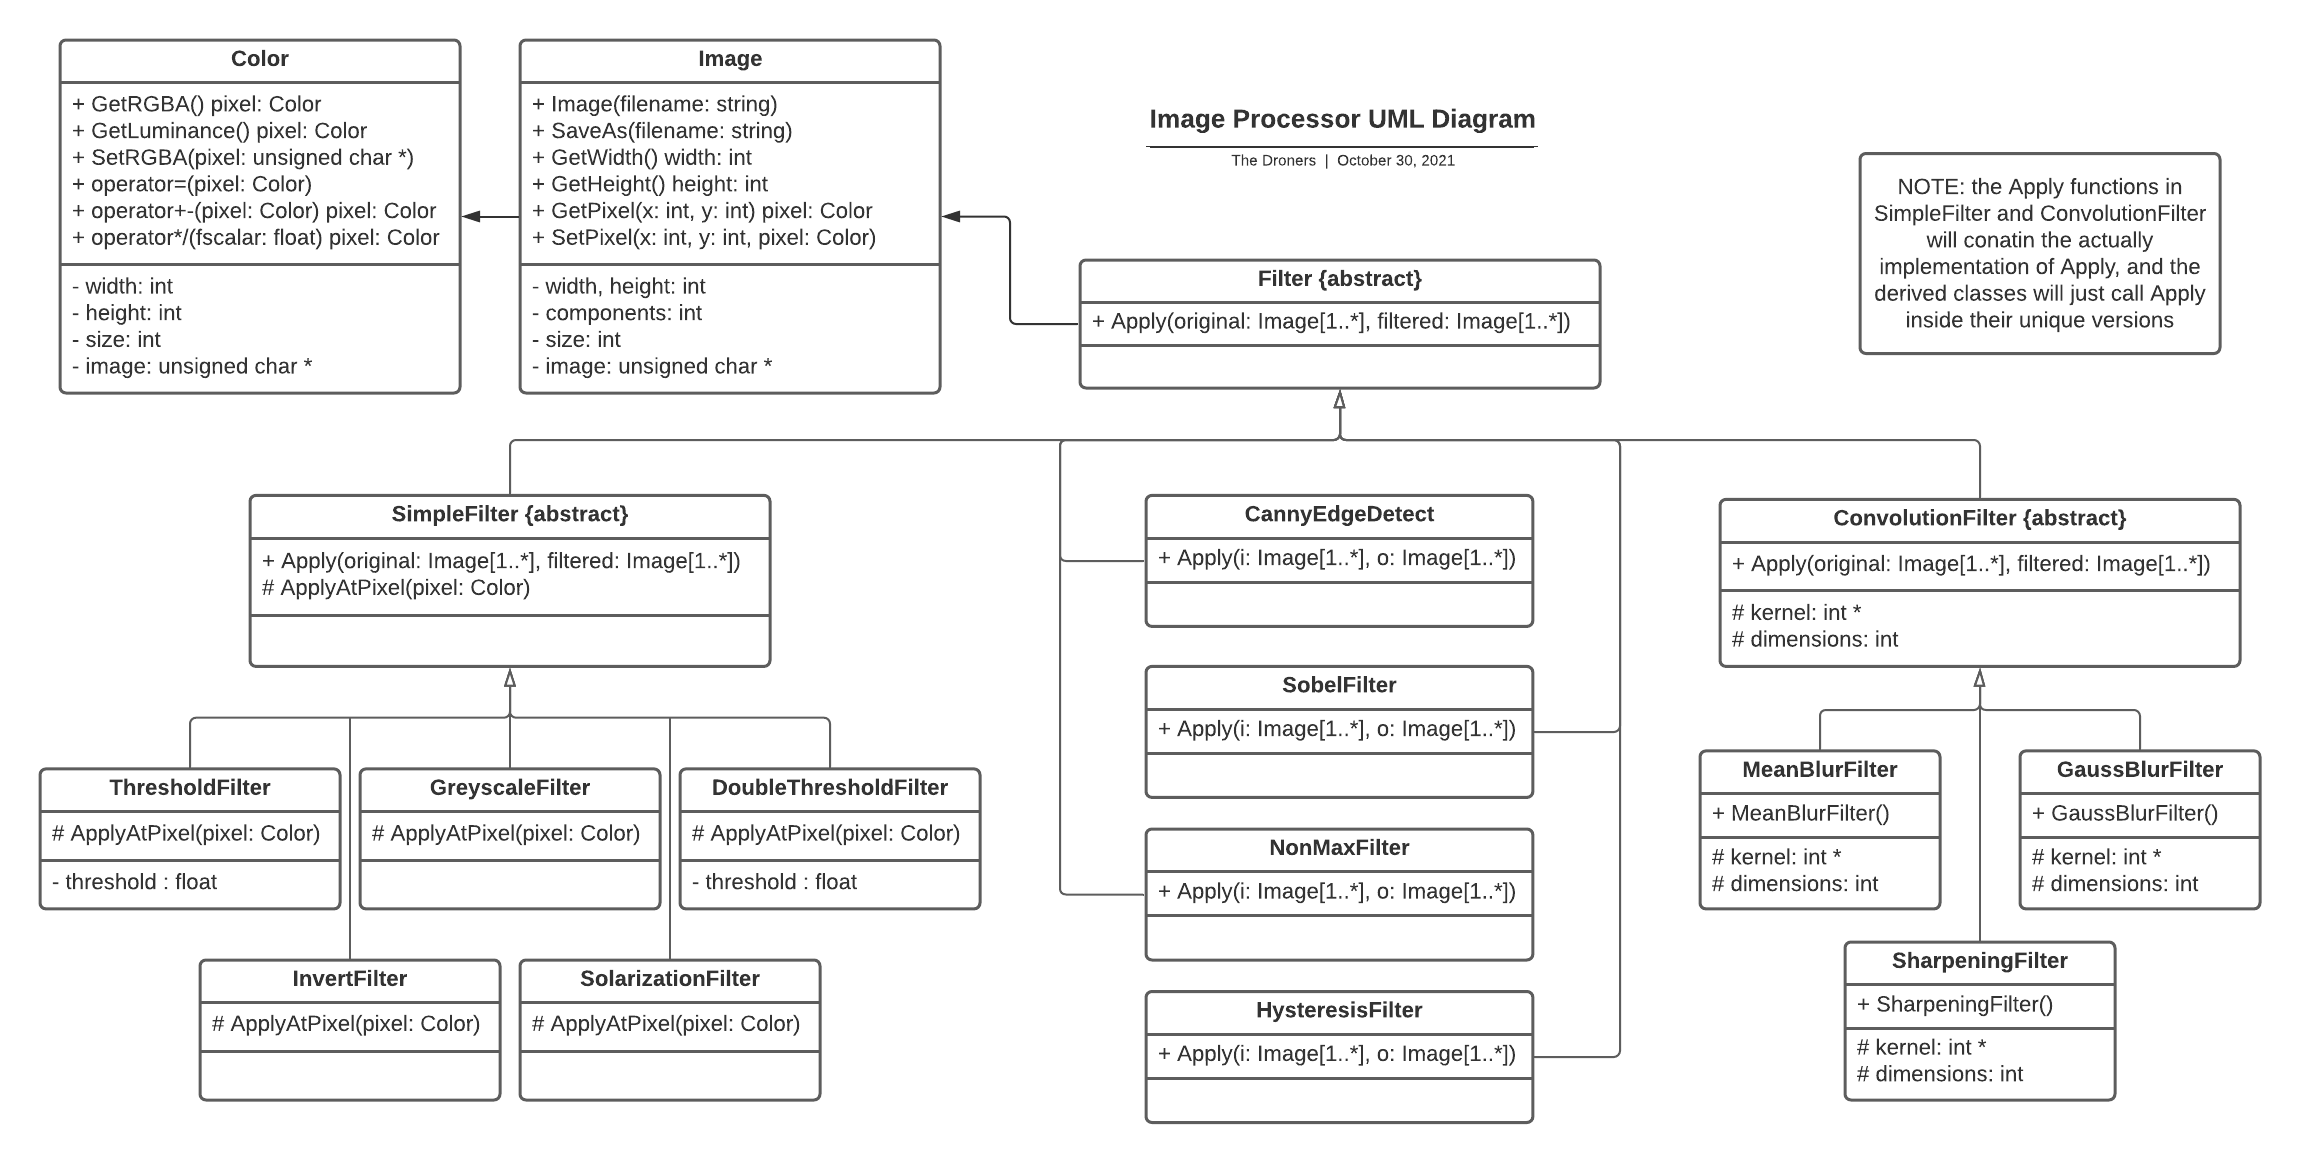
\includegraphics[width=\textwidth]{new.png}

For the actual implementation, my image class was used for processing the image, and I was assigned 
to work on the Sobel Filter as well as the GaussianBlur filter.  I also wrote the Apply functions 
for the SimpleFilter and ConvolutionFilter explained by Gabe. \\

\textbf{Gabe Fendrich:}
In our UML diagram, there are two major classes that inherit from the parent class Filter.  These are 
the abstract classes SimpleFilter and ConvolutionFilter.  Our original intention for this project 
was to make it so that every filter could be implemented as a derived class of one of these two superclasses.  A UML diagram of our initial plan can be   found outlined in the
 
\hyperref[sec:alt]{\textit{Design Alternatives}} section. \\

SimpleFilter iterates through every pixel of the image, calling the ApplyAtPixel function 
of it's respective inherited class, simplifying the implentation of any derived SimpleFilter class and deploying the principle of code reuse.  ConvolutionFilter also iterates through the image, but it instead 
applies a kernel member variable to alter a pixel depending on the luminosity of its neighbors.  This kernel is then 
initialized by the classes that derive ConvolutionFilter, again simplifying their implementation. \\

This approach proved to be more difficult than we initially thought, because certain 
filters don't fit the archetypes of either of Simple or Convolution Filter. There wasn't any shared underlying logic between the four remaining filters, so we decided to have them inherit from Filter and have their own Apply function.  I was responsible for the Hysteresis filter and the Solarization filter. \\

\textbf{Jason Woitalla:}
With the design decisions outlined by Fletcher and Gabe, we already had a pretty SOLID (no pun 
intended) foundation for our code, but I felt something was missing.  When I first started this 
image processing project, I created a Color class that does most of the heavy lifting when it comes 
to altering pixel values.  Utilizing the Color class both standardizes how we interact with pixels, and improves the code readability of changes done to those pixels, making it a no-brainer to add to the design. \\ 

The Color class makes it so that each pixel has a float representation between 0 and 1, which is more 
precise than the one byte pixel representation of an unsigned character array. 
But the main reason for adding this float representation is because some of the filters simply need a larger 
range for the pixel values.  For example, The Sobel filter not only needs numbers larger than one 
to find the intensity gradient (hypotenuse of two pixel values), but also needs negative values 
for the direction gradient (arctan of pixel values).  This is another instance when the Color class is useful, 
as when it comes time the Color class can alter the values back into unsigned 
characters before writing the image. On my end, I was responsible for the 
NonMax Suppression filter, and the PurpleScale.  I also helped Fletcher alter the Image Class so 
it'd work with my Color class. \\

\textbf{Peyton Johnson:}
We already covered all fundamental design decisions that resulted in our finished product, but 
there are still a few smaller coding style decisions we made to add that extra little bit of 
structure to our project that are definitely worth going over. \\

One minor thing is that we decided to use very descriptive terms for our classes, to make sure 
it's obvious what they do.  We also used CamelCase on our classes as a sort of personal design 
choice.  We chose to write filenames in snake\_case and made sure to match header names 
with their corresponding implementation filenames.  We also decided to use header guards 
for all of our classes to make sure the compiler doesn't use multiple instances of a header.  Our 
guards are written in all caps and snake case as another one of our design decisions. \\

On the topic of namespaces, we decided it'd be best to avoid using them for now \cite{namespace}.
At this point, our project is intended for processing images, but we may create one large 
namespace for the whole Filter class hierarchy later when we introduce new aspects to our project.  
As for what I contributed to the design and the project overall, I wrote the doxygen documtentation 
outline as well the CannyEdgeDetect filter and color inversion filter. \\



\textbf{Luke Wiskus:}
With a good stucture of our classes, loose coupling, high cohesion, and code that's closed to change 
and open to extension, we seemed to have succeeded in everything we wanted to do.  There was just 
one small problem though - our files were a mess.  We had a Makefile that could 
compile everything just fine, but there was a single folder containing all of our headers, source files 
and object files.  So every time we wanted to add a filter, that's 3 new files in our already packed 
project directory. \\

To solve this problem, we decided to make changes to our Makefile.  With some trial and error, we were 
able to compartmentalize our files.  We now have a directory called "include" which contains all of our 
headers.  We have a "src" directory for our source and object files.  Finally, our actual image\_processor 
output executable gets dropped in the main project directory where the Makefile is, making 
everything much easier to manage.  For this project, I was responsible for setting up the DoubleThreshold 
filter and SharpeningFilter, as well as the git repository and issue branches for everyone to work on.